%% LyX 2.1.4 created this file.  For more info, see http://www.lyx.org/.
%% Do not edit unless you really know what you are doing.
\documentclass[a4paper,twoside,british,cleardoublepage=empty,BCOR15mm,DIV12]{scrreprt}
\usepackage{amsmath}
\usepackage{tgtermes}
\usepackage{tgheros}
\usepackage{tgcursor}
\usepackage{newtxmath}
\usepackage[T1]{fontenc}
\usepackage[utf8]{inputenc}
\usepackage{babel}
\usepackage{float}
\usepackage{graphicx}
\usepackage[unicode=true,pdfusetitle,
 bookmarks=true,bookmarksnumbered=false,bookmarksopen=false,
 breaklinks=false,pdfborder={0 0 1},backref=false,colorlinks=false]
 {hyperref}

\makeatletter

%%%%%%%%%%%%%%%%%%%%%%%%%%%%%% LyX specific LaTeX commands.
\pdfpageheight\paperheight
\pdfpagewidth\paperwidth

\newcommand{\noun}[1]{\textsc{#1}}
%% Because html converters don't know tabularnewline
\providecommand{\tabularnewline}{\\}
%% A simple dot to overcome graphicx limitations
\newcommand{\lyxdot}{.}

\floatstyle{ruled}
\newfloat{algorithm}{tbp}{loa}[chapter]
\providecommand{\algorithmname}{Algorithm}
\floatname{algorithm}{\protect\algorithmname}

%%%%%%%%%%%%%%%%%%%%%%%%%%%%%% User specified LaTeX commands.
%<-------------------------------společná nastavení------------------------------>
\usepackage[numbers,sort&compress]{natbib} %balíček pro citace literatury  
\usepackage{algorithmic}
\usepackage{color}%kvůli barvám ČVUT
\newcommand{\BibTeX}{{\sc Bib}\TeX}%BibTeX logo
\usepackage{multicol}
\usepackage[overload]{textcase}



%<-----------------------------volání stylů----------------------------------------->
% (znak % je označení komentáře: co je za ním, není aktivní)

%<--------matematické písmo--------------------------------------->

%\usepackage[helvet]{packages/sfmath}%matematika ala helvetica



%<------------------------------záhlaví stránek------------------------------------>
%\usepackage{packages/bc-headings}
\usepackage{packages/bc-fancyhdr}

%<------------------------------hlavičky kapitol------------------------------------>
%\usepackage{packages/bc-neueskapitel}
\usepackage{packages/bc-fancychap}

\makeatother

\begin{document}
~\thispagestyle{empty}\begin{center}\pagenumbering{arabic}\vspace{10mm}


\textsf{\textsc{\noun{\LARGE{}Czech Technical University in Prague}}}\\
\vspace{0.5em}
\textsf{\textsc{\noun{\LARGE{}Faculty of Electrical Engineering}}}\\
\vspace*{1em}
\textsf{\textsc{\noun{\Large{}Department of Cybernetics}}}\vspace{15mm}


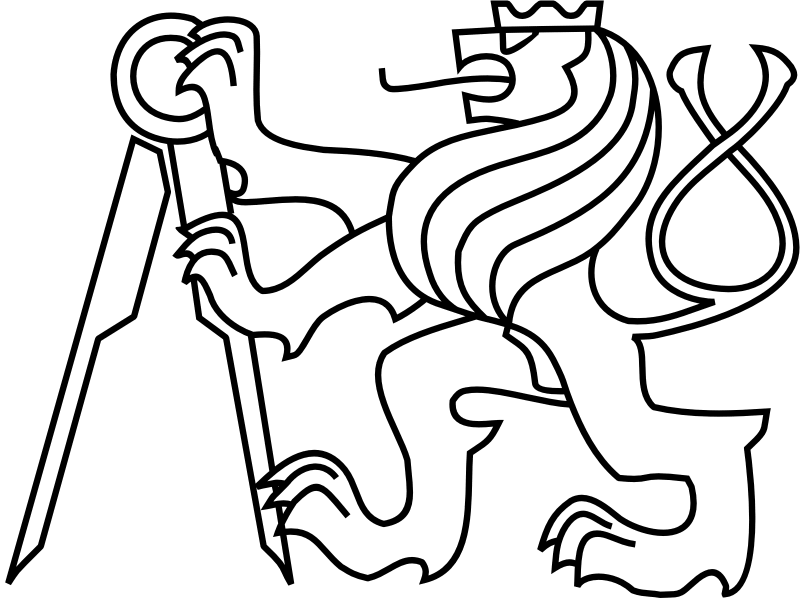
\includegraphics[width=0.3\textwidth]{obrazky/lev}\vspace{15mm}


\textsf{\huge{}BACHELOR THESIS}{\huge \par}

\vspace{15mm}


\textsf{\LARGE{}RRT-path method used for cooperative surveillance
by group of helicopters}{\LARGE \par}

\vspace{10mm}


\end{center} 

\vspace*{\fill}


\vspace{10mm}

\begin{description}
\item [{{\large{}Author:}}] \noindent \textsf{\large{}Matěj Račinský}{\large \par}
\item [{{\large{}Thesis~supervisor:}}] \noindent \textsf{\large{}Dr. Martin
Saska}{\large{}\hfill{}}\textsf{\large{}In Prague,}{\large{} \the\year % nebo doplňte rok vzniku vaší bakalářské práce
}{\large \par}
\end{description}
\clearpage{}

{\small{}\thispagestyle{plain}\addcontentsline{toc}{chapter}{Abstrakt} }{\small \par}

\noindent {\small{}~\vfill{}
}{\small \par}
\begin{description}
\item [{{\small{}Název~práce:}}] \noindent {\small{}Aplikace algoritmu
RRT-path v úloze autonomního dohledu skupinou helikoptér}{\small \par}
\item [{{\small{}Autor:}}] \noindent {\small{}Matěj Račinský}{\small \par}
\item [{{\small{}Katedra~(ústav):}}] \noindent Kate{\small{}dra kybernetiky}{\small \par}
\item [{{\small{}Vedoucí~bakalářské~práce:}}] \noindent Dr. Martin Saska
\item [{{\small{}e-mail~vedoucího:}}] \noindent {\small{}saska@labe.felk.cvut.cz}\\
{\small \par}
\item [{{\small{}Abstrakt}}] \noindent {\small{}V předložené práci studujeme...
Uvede se abstrakt v rozsahu 80 až 200 slov. Lorem ipsum dolor sit
amet, consectetuer adipiscing elit. Ut sit amet sem. Mauris nec turpis
ac sem mollis pretium. Suspendisse neque massa, suscipit id, dictum
in, porta at, quam. Nunc suscipit, pede vel elementum pretium, nisl
urna sodales velit, sit amet auctor elit quam id tellus. Nullam sollicitudin.}{\small \par}
\item [{{\small{}Klíčová~slova:}}] \noindent {\small{}klíčová slova (3
až 5)}\\
{\small \par}
\item [{\rule[0.5ex]{1\linewidth}{1pt}}]~{\small \par}
\item [{{\small{}Title:}}] \noindent {\small{}RRT-path method used for
cooperative surveillance by group of helicopters}{\small \par}
\item [{{\small{}Author:}}] \noindent {\small{}Matěj Račinský}{\small \par}
\item [{{\small{}Department:}}] \noindent {\small{}Department of Cybernetics}{\small \par}
\item [{{\small{}Supervisor:}}] \noindent Dr. Martin Saska
\item [{{\small{}Supervisor's~e-mail~address:}}] \noindent {\small{}saska@labe.felk.cvut.cz}\\
{\small \par}
\item [{{\small{}Abstract}}] \noindent {\small{}In the present work we
study ... Uvede se anglický abstrakt v rozsahu 80 až 200 slov. Lorem
ipsum dolor sit amet, consectetuer adipiscing elit. Ut sit amet sem.
Mauris nec turpis ac sem mollis pretium. Suspendisse neque massa,
suscipit id, dictum in, porta at, quam. Nunc suscipit, pede vel elementum
pretium, nisl urna sodales velit, sit amet auctor elit quam id tellus.
Nullam sollicitudin. Donec hendrerit. Aliquam ac nibh. Vivamus mi.
Sed felis. Proin pretium elit in neque. Pellentesque at turpis. Maecenas
convallis. Vestibulum id lectus. }{\small \par}
\item [{{\small{}Keywords:}}] \noindent {\small{}klíčová slova (3 až 5)
v angličtině}{\small \par}
\end{description}
\cleardoublepage{}\thispagestyle{empty}~{\small{}\addcontentsline{toc}{chapter}{Zadání
práce} }{\small \par}

\thispagestyle{plain}

{\small{}%\setcounter{page}{3} % nastavení číslování stránek
\ }{\small \par}

\noindent {\small{}\vfill{}
 % nastavuje dynamické umístění následujícího textu do spodní části stránky
~}{\small \par}

\noindent {\small{}Prohlašuji, že jsem svou bakalářskou práci napsal(a)
samostatně a výhradně s použitím citovaných pramenů. Souhlasím se
zapůjčováním práce a jejím zveřejňováním.}{\small \par}

{\small{}\bigskip{}
}\noindent {\small{} V Praze dne \today\hspace{\fill}Jméno Příjmení
+ podpis}\\
{\small{} % doplňte patřičné datum, jméno a příjmení
}{\small \par}

{\small{}%%%   Výtisk pak na tomto míste nezapomeňte PODEPSAT!
%%%                                         *********
}{\small \par}

{\small{}\tableofcontents{}% vkládá automaticky generovaný obsah dokumentu
}{\small \par}


\chapter[Motivation]{Motivation}


\chapter[Algorithm]{Algorithm\label{chap:Algorithm}}

The basis of the whole algorithm is shown in \ref{alg:Basis-of-whole}
in the pseudocode.

\begin{algorithm}
\caption{The basis of whole algorithm\label{alg:Basis-of-whole}}


\begin{algorithmic}[1]

\STATE map := configuration.getMap();

\STATE map := amplifyObstacles(map);

\STATE nodes := mapToNodes(map);

\STATE paths := createGuidingPaths(nodes);

\STATE rrtPath := rrtPath(paths, map, nodes);

\STATE lastState := getBestFitness(rrtPath, map);

\STATE path := getPath(lastState);

\STATE path = straightenCrossingTrajectories(path);

\STATE path := resamplePath(path, map);

\STATE path := optimizePathByDubins(path, map);

\STATE savePath(path);

\end{algorithmic}
\end{algorithm}


The configuration variable is instance of the Configuration class,
which holds all configuration data, including a selected map. The
map holds all Areas of Interest (AoI) and obstacles. All obstacles
and AoIs are represented as rectangles now.

The purpose of the path finding is to find the shortest feasible paths,
but real UAVs need to have some minimal distance to obstacles due
to weather conditions, sensor errors and other aspects. To solve this
issue, every obstacle is amplified before the whole path finding algorithm
on line 2. This minimal distance to obstacles allows UAVs to follow
their trajectories safely.

The 3rd line represents the discretization of the map to the graph.
The discretization divides the map to squares with size set in the
configuration and each square is represented by a graph node. In this
graph, there are 4 types of nodes: Free, Obstacle, UAV and Goal. If
the whole square or its part is covered by an obstacle, the corresponding
node has the type Obstacle. If the whole square or its part is covered
by an AoI, then the corresponding node has type Goal. If the square
contains an UAV, the corresponding node has type UAV and rest of squares
have corresponding nodes with type Free. 

Edges in this graph are only between nodes of neighbouring squares,
so each node has maximally 8 edges. Obstacle nodes do not have any
edges.

After converting the map to nodes, the optional grouping of goals
for guiding path can be turned on. I will cover the grouping in chapter
\ref{chap:Grouping-of-goals}.

The 4th line represents the calculation of the guiding paths for RRT-Path
algorithm using the A{*} algorithm with modified cost function. The
modification will be covered in section \ref{sec:Guiding-path}.

On the 5th line the RRT-Path algorithm takes place. This function
returns a structure with a tree with a root at the starting position
of UAVs and with an array containing leaves of this three, where all
UAVs are in Areas of Interest. 

The leaf, where UAVs have the best coverage of AoI, is chosen on line
6. The quality of the coverage is determined by the cost function,
which will be mentioned later.\marginpar{todo: možná sem odkaz na kapitolu}

On the 6th line the path is built from the last state.

On the 8th line there is an optional preparation before the optimization
using Dubins curves. In the preparation, all crossings of paths of
individual UAVs are straightened, so UAVs do not cross other trajectories
during the whole path. During the implementation of this method some
complications appeared, which are covered in the chapter \ref{chap:Paths-straightening},
and thus the row was removed from the final version of the algorithm. 

On the 9th line, the re-sampling of the path is made, mainly due to
requirements of real UAVs, which are mentioned in chapter \ref{chap:Path-resampling}.

On the 10th line there is the optimization by Dubins curves. The optimization
is covered in chapter \ref{chap:Dubins-curves}.

The last line represents persisting of the path to a file for usage
of path by different programs. Path is persisted to JSON, due to convenience
of the JSON format. JSON is smaller than XML and can be easily parsed
by all widely used programming languages. Path is also persisted to
CSV format, so it can be loaded to MATLAB and then loaded into real
UAVs.


\chapter[Grouping of goals for the guiding path]{ Grouping of goals for the guiding path \label{chap:Grouping-of-goals}}

During this processing of the map (method MapProcessor::getEndNodes
in codebase) all AoIs are grouped to one big AoI, which is the smallest
rectangle covering all AoIs. 

If this modification is turned on, then instead of one goal for every
AoI (node in the middle of AoI rectangle is considered as a goal node),
only one goal is used for all AoIs. This prevents swarm to split because
the whole swarm has only one guiding path. The relative localization
is the main reason to have only one big swarm instead of more smaller
swarms is that a smaller swarms (or individual UAVs in case of the
same count of AoI and UAVs). Advantages of relative localization are
more significant when we have only one swarm.

\marginpar{todo: rozepsat vytváření shluknutého cíle a jak z něj najdu goal node
pro a star}

Maps with goals and obstacles are shown in figures \ref{fig:Map-with-goals}
and \ref{fig:Maps-with-goals}. Goals are coloured green colour and
obstacles grey.

This approach has the following advantage: when individual AoIs are
near to a global goal of the whole group, as seen in \ref{fig:Maps-with-goals},
then the whole swarm follows one guiding path without any splitting,
which makes the RRT-Path run faster and also the advantage of relative
localization is included. 

The disadvantage of this method is that when individual AoIs have
a bigger distance from each other than can be covered by UAVs then
this approach totally fails, because RRT-Path, which is much faster
than RRT, has goal very distant from AoIs, as can be seen in \ref{fig:Map-with-goals}.\marginpar{rozdělit na více vět }

\begin{figure}
\begin{centering}
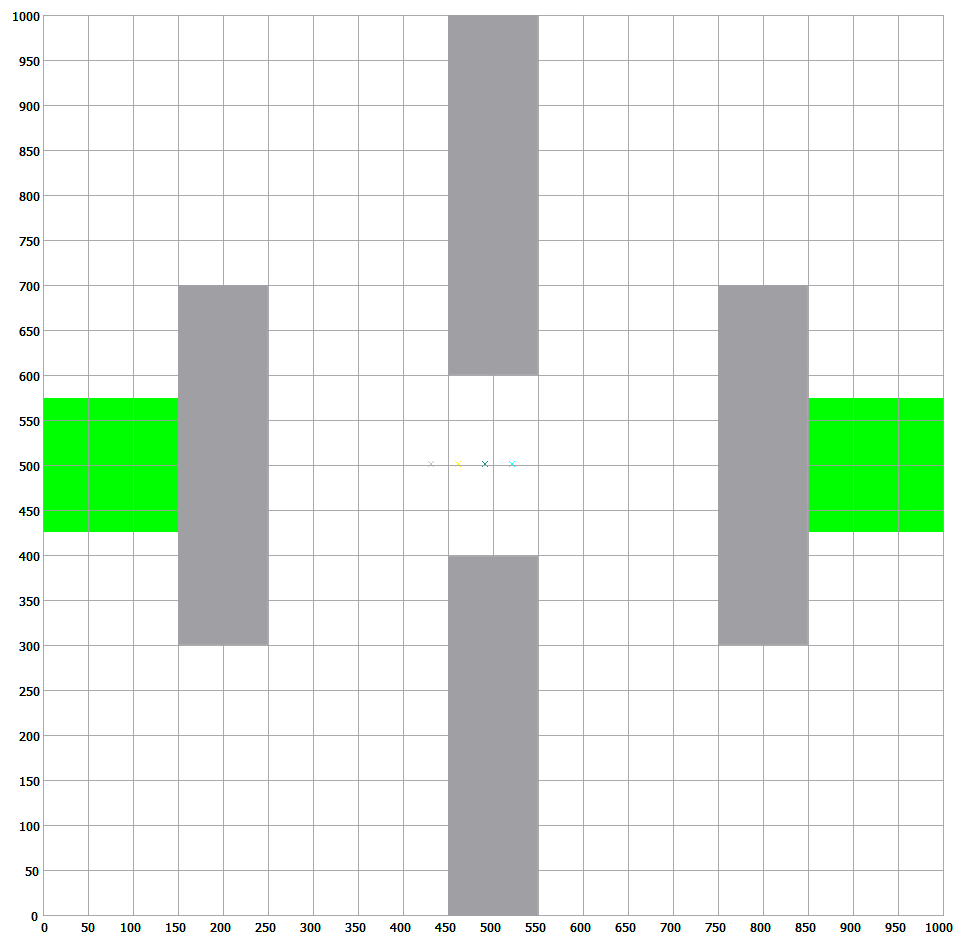
\includegraphics[scale=0.3]{obrazky/map1}
\par\end{centering}

\caption{Map with goals unsuitable for grouping \label{fig:Map-with-goals}}
\end{figure}


\begin{figure}
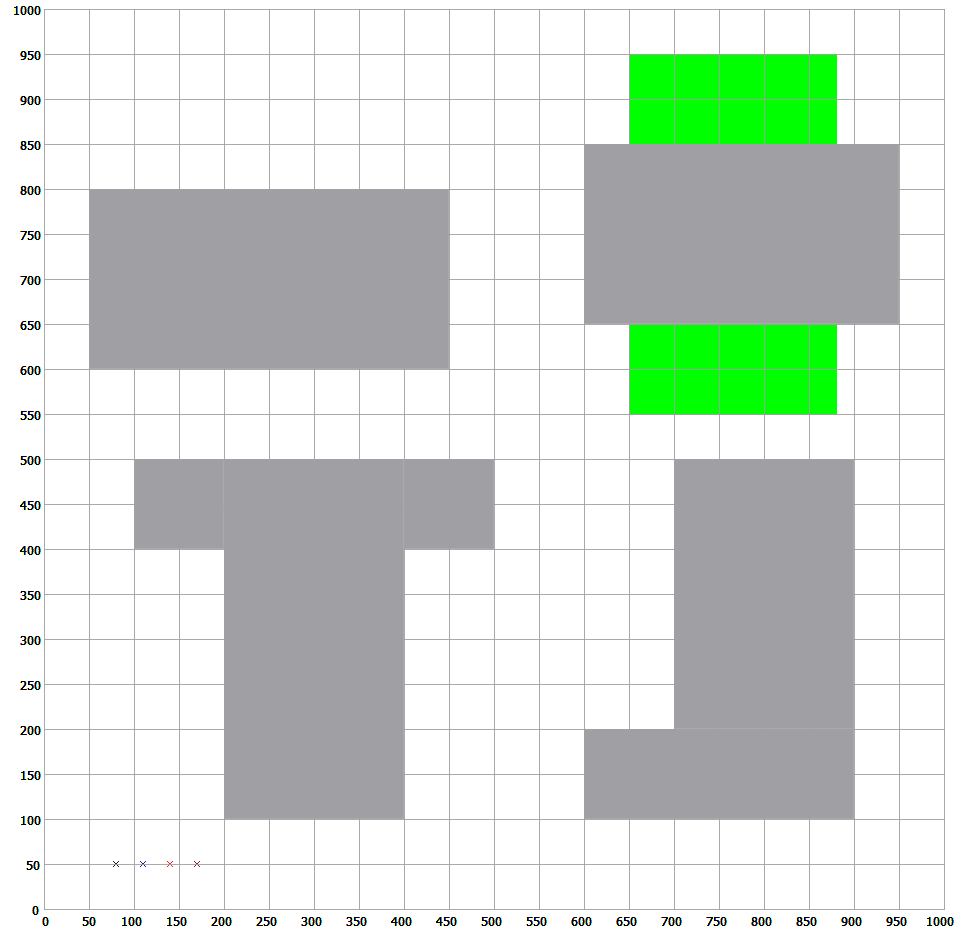
\includegraphics[scale=0.3]{obrazky/map2}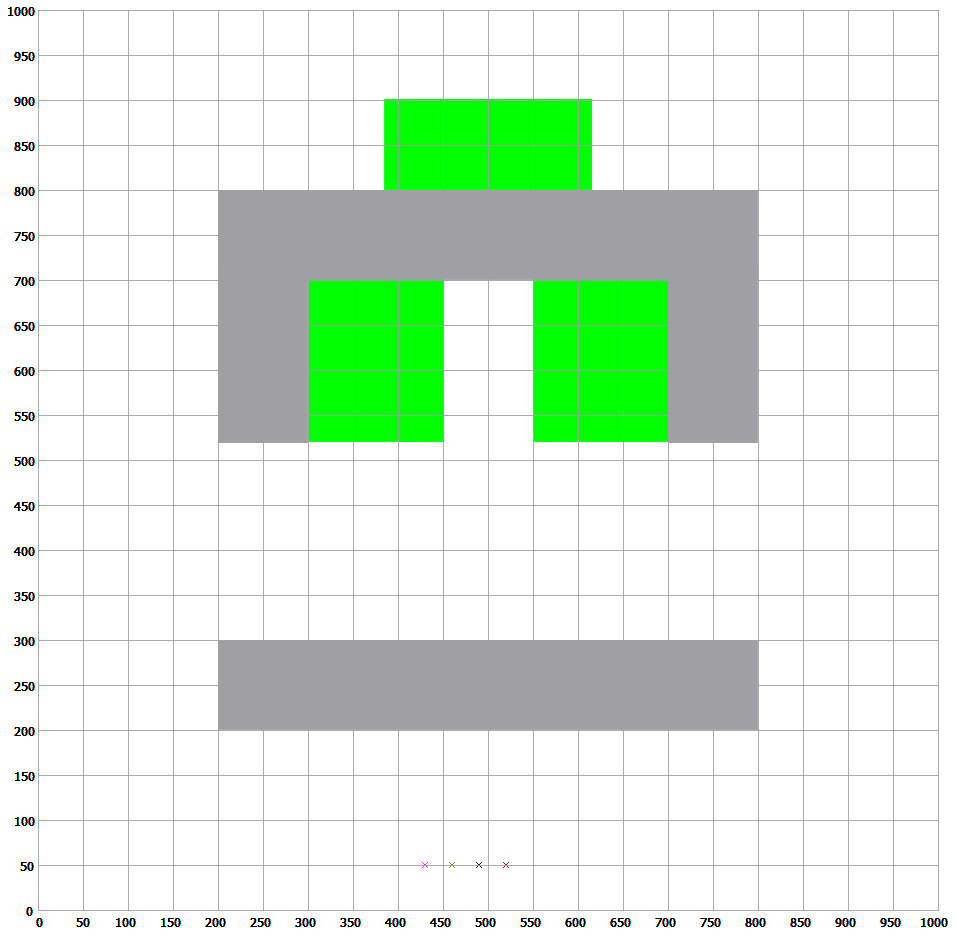
\includegraphics[scale=0.3]{obrazky/map5}

\caption{Maps with goals suitable for grouping \label{fig:Maps-with-goals}}
\end{figure}



\chapter[RRT-Path]{RRT-Path}

This chapter will cover brief introduction of RRT-Path algorithm.
But before that, we need to define RRT algorithm which RRT-Path is
based on.


\section{Rapidly Exploring Random Tree}

Rapidly Exploring Random Tree, also abbreviated as RRT, introduced
by LaValle\cite{LaValle1998} in 1998, is non-deterministic algorithm
for motion planning, used to search non-convex spaces by randomly
building space-filling tree. The RRT method builds a tree $T$ rooted
at $q_{start}$. The basic RRT algorithm works as follows. In each
iteration, a random sample $q_{rand}$ is chosen from $C$ and the
nearest node $q_{near}$ in the tree to $q_{rand}$ is found. The
node $q_{near}$ is expanded using a local planner to obtain a set
of new configurations reachable from $q_{near}$. The nearest configuration
towards q is selected from this set and added to the tree. The edge
from q near rand to the newly added configuration contains control
inputs used by the local planner to reach the new configuration. The
algorithm terminates if the distance between a node in the tree and
$q_{goal}$ is less than $d_{goal}$ or after $I_{max}$ of planning
iterations. \cite{Vonasek2015} The basis of RRT is listed in algorithm
\ref{alg:RRT-algorithm}. In RRT algorithm, configurations on the
third line have uniform distribution.

\begin{algorithm}
\caption{RRT algorithm\label{alg:RRT-algorithm}}


\textbf{Input: }Configurations $q_{alert}$ and $q_{goal}$, maximum
number of iterations $I_{max}$, maximum distance to goal $d_{goal}$

\textbf{Output:} Trajectory $P$ or failure

\begin{algorithmic}[1]

\STATE $T.add\left(q_{start}\right);$ // create new tree and add
initial conguration q in it

\STATE \textbf{for} iteration:=1:I \textbf{do} 

\STATE ~$q_{rand}$ := getRandomConfiguration($C$);

\STATE ~$q_{near}$ := nearest node in tree $T$ to q ;

\STATE ~expandTree($q_{rand}$,$q_{near}$);

\STATE ~$d$ = distance from tree $T$ to $q_{goal}$ ;

\STATE ~\textbf{if} d < d \textbf{then}

\STATE ~~P = extract trajectory from $q_{start}$ to $q_{rand}$;

\STATE ~~return P;

\STATE ~\textbf{end}

\STATE \textbf{end}

\STATE return failure; // no solution was found within K iterations
start

\end{algorithmic}
\end{algorithm}



\section{RRT-Path}

RRT-Path, introduced by Vonásek \cite{Vonasek2015} in 2015, is an
improved version of RRT featuring preprocessing of configuration space.
RRT-Path enables UAVs to manoeuvre around obstacles and find way in
narrow passages. Before running RRT algorithm, the guiding path from
$q_{start}$ to $q_{goal}$ is found and sampled. One of inputs to
RRT-Path algorithm is the probability $p\left(guided\right)$. In
the main loop of the algorithm, obtaining of the random configuration
is modified. Instead of random configuration with uniform distribution,
configuration around the $q_{i}$is selected with probability $p\left(guided\right)$.

Let $G$ be the guiding path and $\left(q_{start},q_{1},q_{2},...,q_{goal}\right)\text{\ensuremath{\in}}G$
the points of the guiding path, where $q_{i}\text{\ensuremath{\in}}C_{free}$.
In the beginning, $q_{i}=q_{1}$, so random point is selected from
area around the point $q_{1}$ with probability $p\left(guided\right)$.
When the leaves of the searching tree reach distance lower than $r_{dist}$to
the $q_{i}$, then the next point of the guiding path will be used
instead of $q_{i}$, so $q_{i}:=q_{i+1}$. This continues until $q_{goal}$
is reached, which means the RRT-Path algorithm ends.


\section{Guiding path\label{sec:Guiding-path}}

The guiding path is obtained by transferring the map to graph representation
and then path is found using the graph-search algorithms. The map
can be transferred to graph representation by using the Voronoi diagram,
visibility graph or by discretization to a grid representation. 

Then the path can be found by using Dijkstra algorithm or A{*} algorithm.
In this thesis, the A{*} algorithm has been used because of its ability
to find optimal path and easy calculation of heuristic function is
Euclidean space.

The classic cost function of node $q_{i}$ in A{*} algorithm is $f\left(q_{i}\right)=g\left(q_{i}\right)+h\left(q_{i}\right)$.
The $g\left(q_{i}\right)$ is sum of costs of all edges in shortest
path between nodes and $q_{init}$ and $q_{i}$. The $h\left(q_{i}\right)$
is heuristic estimate of distance between $q_{i}$ and $q_{goal}$.
In Euclidean space, it is calculated as $h\left(q_{i}\right)=\left\Vert q_{i}-q_{goal}\right\Vert $.
This algorithm uses a modified cost function and in addition to a
cost function of the A{*} algorithm. The modified cost function is
$f\left(q_{i}\right)=g\left(q_{i}\right)+h\left(q_{i}\right)+j\left(q_{i}\right)$,
where $j\left(q_{i}\right)$ is integer representing the nearness
to the nearest obstacle. For example, it can be $j\left(q_{i}\right)=\frac{const}{\left\Vert q_{i}-nearest\,obstacle\right\Vert }$,
where $const$ is weight of the $j\left(q_{i}\right)$ and expresses
how much obstacles should be avoided with respect to length of the
whole path.


\chapter[Paths straightening]{Paths straightening \label{chap:Paths-straightening}}

RRT-Path algorithm checks crossing paths between neighbouring states,
so between nth state and n+1-th \marginpar{todo: zjistit, jak je to správně anglicky}
state no trajectories are crossing each other. But between states
trajectories are still crossing. In this image \ref{fig:Crossing-paths}
is shown path found by RRT-Path. Every colour marks one state in RRT-Path.
As we can see, check in algorithm prevents from crossing path between
neighbouring states, but crossing of paths in different times can
not be easily prevented. We can see in image, that paths cross between
points J (yellow), M (light green) and H (orange), K (yellow), so
there is no easy approach to prevent path collisions between n-2-th
state and nth state. Optimization by Dubins curves shortens trajectory
of UAVs, so UAVs could be in these trajectories in different time,
so there could be collisions after optimization. Another complication
occurs, when time difference between two states is too low, then UAVs
could collide, because in reality UAV can not follow path precisely,
but only with some errors.

\begin{figure}
\caption{Crossing paths \label{fig:Crossing-paths}}


\centering{}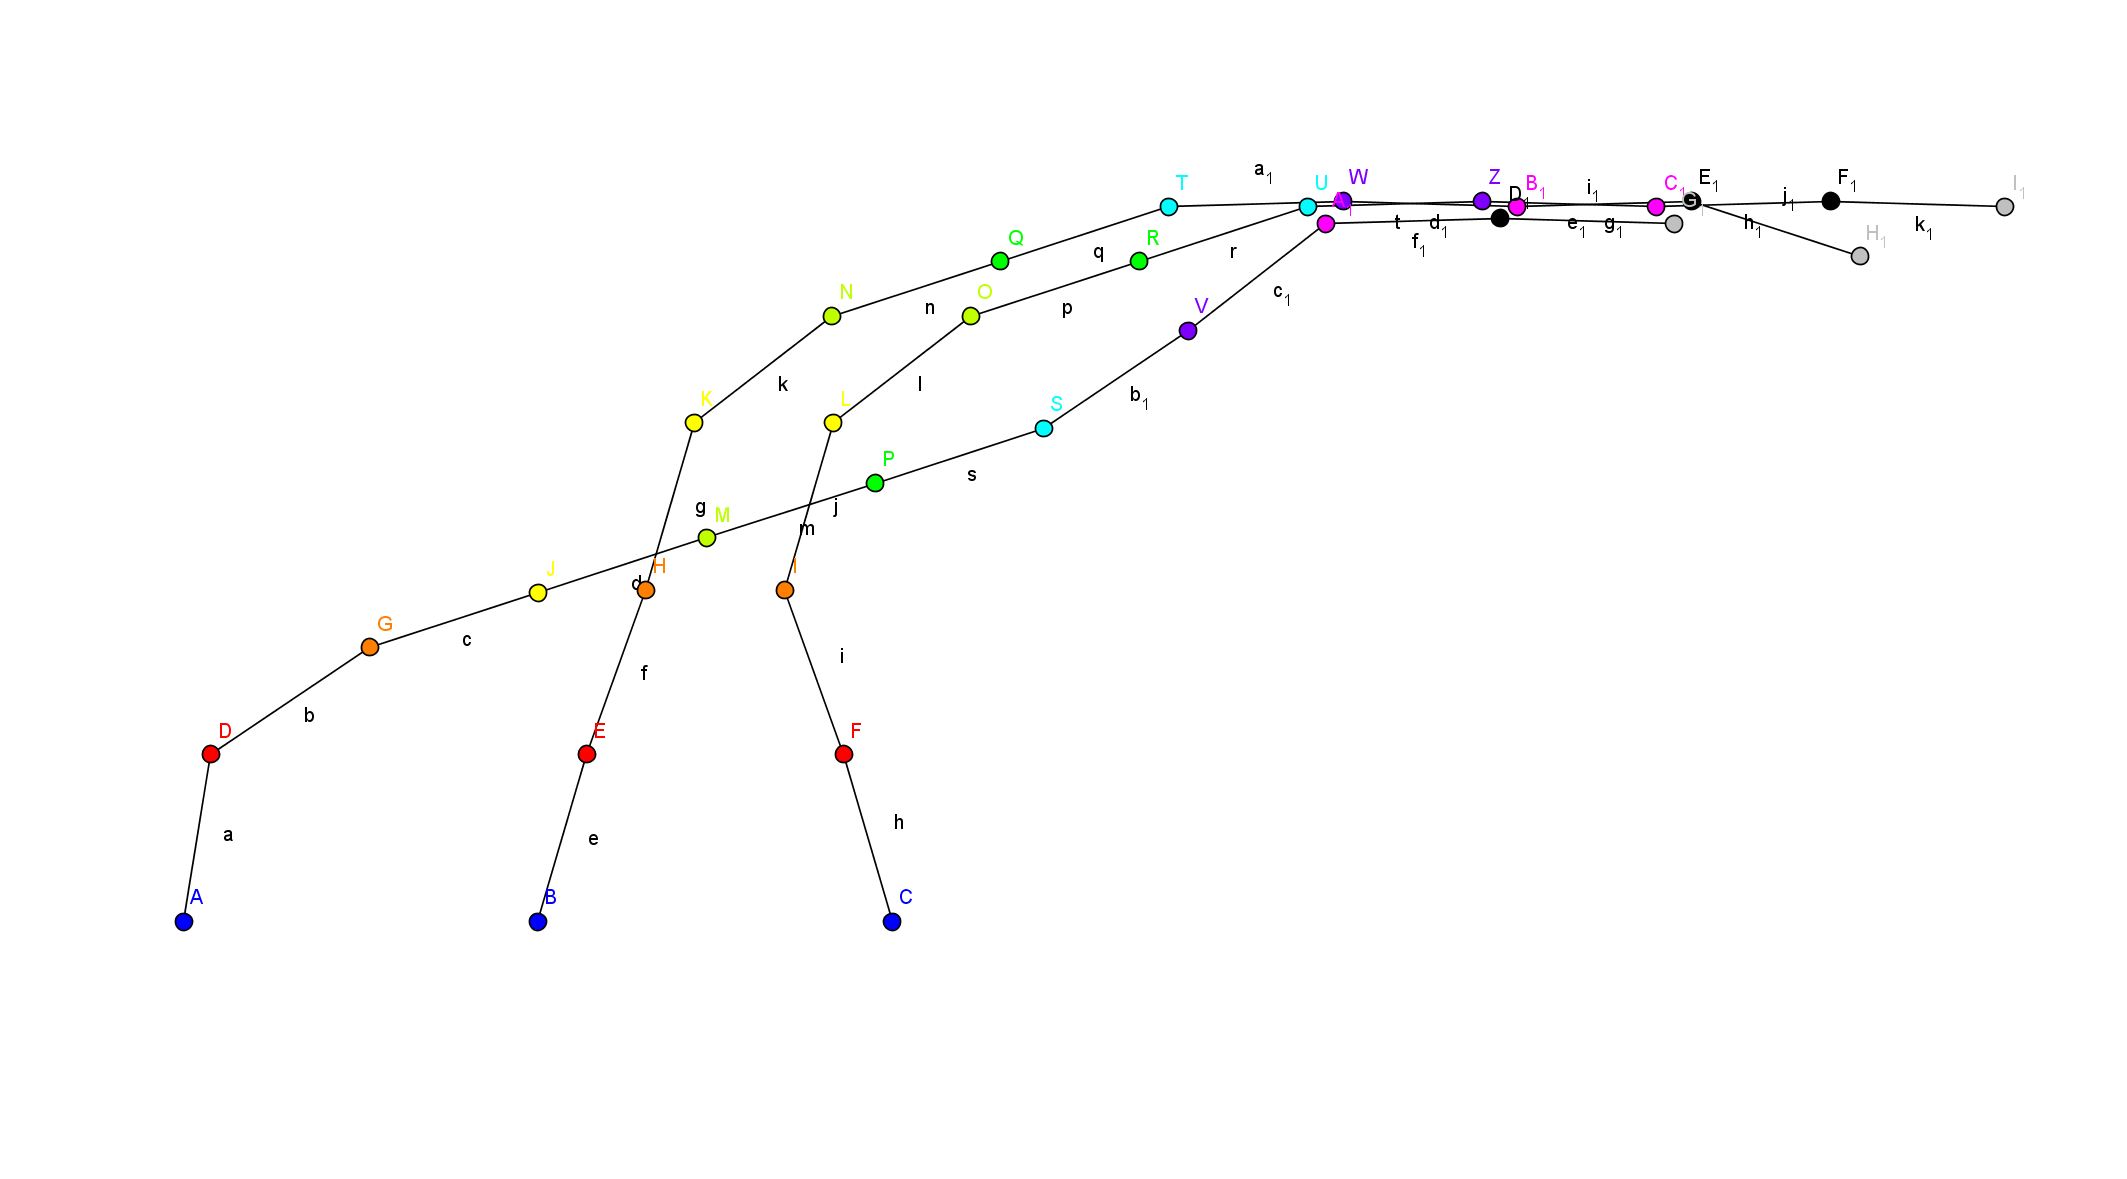
\includegraphics[scale=0.3]{obrazky/crossingPathReal1}
\end{figure}
I tried to straighten crossing trajectories, but all attempts failed.
Straightening was done by switching parts of crossing paths from the
earliest crossing state to end. But then paths had different lengths,
which was unsuitable for path planning for swarm. This can be done
by adding ``waiting'' points, points in different state but with
same position in different time. But then is really hard to straighten
longer path with many crossings (this path is really short, paths
in other maps are much longer and more complicated). For motion model
with inertia is also really hard to deal with waiting states, which
complicates following of straightened trajectories. Due to all complications
mentioned above, this part was removed from algorithm. But it is possible
to add it, when better approach will be found.


\chapter[Motion model]{Motion model}

The RRT-Path algorithm is universal and works without motion model,
which is fine for holonomic robot, but usage of motion model allows
us to find path more feasible for swarm of UAVs than without using
of holonomic robot. For this purpose, car like model was chosen. Differential
equations of motion model in 3D from \cite{MartinSaskaPreucil} are
\begin{equation}
\begin{array}{ccc}
\dot{x}\left(t\right) & = & v\left(t\right)\sin\varphi\left(t\right)\\
\dot{y}\left(t\right) & = & v\left(t\right)\cos\left(t\right)\\
\dot{z}\left(t\right) & = & w\left(t\right)\\
\dot{\varphi}\left(t\right) & = & K\left(t\right)v\left(t\right)
\end{array}
\end{equation}
where $x\left(t\right),y\left(t\right),z\left(t\right)$ are coordinates
of UAV, $\varphi\left(t\right)$ represents heading of UAV, $v\left(t\right)$
is forward velocity, $K\left(t\right)$ is curvature, $w\left(t\right)$
is ascent velocity. $\begin{bmatrix}K\left(t\right) & w\left(t\right) & v\left(t\right)\end{bmatrix}$
represent input vector of motion model. Differential equations are
useful for representation in equations, but not useful for computer
algorithm. For usage in algorithm are better difference equations
instead of differential equations. When inputs are held constant in
each time interval between two time steps, difference equations are
\begin{equation}
\begin{array}{ccc}
x\left(k+1\right) & = & \begin{cases}
if\,K\left(k+1\right)\neq0\\
x\left(k\right)+\frac{1}{K\left(k+1\right)}\left(\sin\left(\varphi\left(k\right)+K\left(k+1\right)v\left(k+1\right)\Delta t\left(k+1\right)\right)-\sin\left(\varphi\left(k\right)\right)\right)\\
if\,K\left(k+1\right)=0\\
x\left(k\right)+v\left(k+1\right)\cos\left(\varphi\left(k\right)\right)\Delta t\left(k+1\right)
\end{cases}\\
y\left(k+1\right) & = & \begin{cases}
if\,K\left(k+1\right)\neq0\\
y\left(k\right)-\frac{1}{K\left(k+1\right)}\left(\cos\left(\varphi\left(k\right)+K\left(k+1\right)v\left(k+1\right)\Delta t\left(k+1\right)\right)-\cos\left(\varphi\left(k\right)\right)\right)\\
if\,K\left(k+1\right)=0\\
y\left(k\right)+v\left(k+1\right)\sin\left(\varphi\left(k\right)\right)\Delta t\left(k+1\right)
\end{cases}\\
z\left(k+1\right) & = & z\left(k\right)+w\left(k+1\right)\Delta t\left(k+1\right)\\
\varphi\left(k+1\right) & = & \varphi\left(k\right)+K\left(k+1\right)v\left(k+1\right)\Delta t\left(k+1\right)
\end{array}
\end{equation}



\chapter[Dubins curves]{Dubins curves\label{chap:Dubins-curves}}

Dubins curves, also called Dubins manoeuvrers or Dubins path were
published by Lester Eli Dubins in 1957 \cite{Dubins1957}. Dubins
path is optimal path for car like motion model. Path is optimal, when
car moves at constant forward speed. The other important constraint
is the maximum steering angle $\phi_{max}$, which results in a minimum
turning radius$\rho_{min}$. As the car travels, consider the length
of the curve in ${\cal W}=\mathbb{R}^{2}$ traced out by a pencil
attached to the centre of the car. The task is to minimize the length
of this curve as the car travels between any $q_{I}$ and $q_{G}$.
Due to $\rho_{min}$, this can be considered as a bounded-curvature
shortest-path problem. If $\rho_{min}=0$, then there is no curvature
bound, and the shortest path follows a straight line in $\mathbb{R}^{2}$.
In terms of a cost function, the criterion to optimize is

\begin{equation}
\ensuremath{{\displaystyle L(\tilde{q},\tilde{u})=\int_{0}^{t_{F}}\sqrt{\dot{x}(t)^{2}+\dot{y}(t)^{2}}dt}}
\end{equation}
, where $t_{F}$ is the time at which $q_{G}$ is reached, and a configuration
is denoted as $q=(x,y,\theta)$, $\tilde{x}_{t}$ denotes the function
$\tilde{x}_{t}:[0,t]\rightarrow X$, which is called the state trajectory
(or state history). This is a continuous-time version of the state
history, which was defined previously for problems that have discrete
stages. Similarly, $\tilde{u}_{t}$ denotes the action trajectory
(or action history),. If $q_{G}$ is not reached, then it is assumed
that $L(\tilde{q},\tilde{u})=\infty$. \cite{LaValle2006}

When considering constraints of inputs (actions) for motion model,
the system can be simplified to

\begin{equation}
\begin{array}{ccc}
\dot{x} & = & \cos\theta\\
\dot{y} & = & \sin\theta\\
\dot{\theta} & = & u
\end{array}
\end{equation}


in which $u$ is chosen from the interval $U=\left\{ -\tan\phi_{max},0,\tan\phi_{max}\right\} $.
For simplicity, assume that $\tan\phi=1$. The following results also
hold for any $\phi_{max}\in(0,\pi/2)$. 

\begin{table}
\caption{The three motion primitives from which all optimal curves for the
Dubins car can be constructed. \label{tab:The-three-motion}}


\begin{tabular}{|c|c|}
\hline 
Symbol & Steering u\tabularnewline
\hline 
\hline 
L & -1\tabularnewline
\hline 
S & 0\tabularnewline
\hline 
R & 1\tabularnewline
\hline 
\end{tabular}
\end{table}


It was shown in \cite{Dubins1957} that between any two configurations,
the shortest path for the Dubins car can always be expressed as a
combination of no more than three motion primitives. Each motion primitive
applies a constant action over an interval of time. Furthermore, the
only actions that are needed to traverse the shortest paths are $u\in\{-1,0,1\}$.
The primitives and their associated symbols are shown in \ref{tab:The-three-motion}.
The $S$ primitive drives the car straight ahead. The $L$ and $R$
primitives turn as sharply as possible to the left and right, respectively.
Using these symbols, each possible kind of shortest path can be designated
as a sequence of three symbols that corresponds to the order in which
the primitives are applied. Let such a sequence be called a word .
There is no need to have two consecutive primitives of the same kind
because they can be merged into one. Under this observation, ten possible
words of length three are possible. Dubins showed that only these
six words are possibly optimal:

\begin{equation}
\ensuremath{{\displaystyle \{LRL,\;RLR,\;LSL,\;LSR,\;RSL,\;RSR\}.}}
\end{equation}


The shortest path between any two configurations can always be characterized
by one of these words. These are called the Dubins curves.


\section[Optimization using Dubins curves]{Optimization using Dubins curves}

Because of the fact that Dubins curves provide us optimal trajectory,
they can be used to optimize trajectory found with RRT-Path algorithm.

For only one UAV, the situation is quite simple and optimization works
as follows.

Two random points of trajectory are chosen and Dubins curves are calculated
between them. If calculated curves do not collide with the obstacles,
they are used instead of original trajectory between chosen points.
This points choosing and trajectory replacing is repeated until the
whole trajectory can not be shortened more and thus is optimal.

In real situation, we do not know whether found trajectory is optimal
or not, so we need to determine conditions for stopping the optimization.
The optimization is stopped if the trajectory is not shortened after
many (e. g. 150) iterations or optimization is too slow and path is
shortened only by small distances (e. g. shortening by 5\% per 1000
iterations). 

But in swarm, the situation is complicated because of relative localization
and minimal and maximal distances between individual UAVs. 

So the algorithm must be modified. Dubins curves must be sampled in
same frequency as rest of trajectory (this is frequency of RRT-Path
algorithm or higher frequency when path is being re-sampled) and each
point has to be validated for feasibility in terms of minimal and
maximal distance from another UAVs. So the curves can be used only
when all trajectories between minimal and maximal distance of relative
localization.


\subsection[One UAV demonstration]{One UAV demonstration}

In \ref{fig:One-UAV-before} we have trajectory of one UAV found by
RRT-Path algorithm in map with one obstacle marked by dark grey rectangle.
Obstacle amplification is marked by light grey rectangle. In \ref{fig:One-UAV-after}
we can see optimal path found using Dubins curves. The resulting path
consists of many Dubins curves and it was obtained by algorithm mentioned
above. Random points have been replaced by Dubins curves and after
many iterations, optimal path was found.

\begin{figure}


\caption{One UAV before Dubins curves optimization\label{fig:One-UAV-before}}


\centering{}\includegraphics[scale=0.6]{obrazky/oneUAV\lyxdot json}
\end{figure}


\begin{figure}


\caption{One UAV after Dubins curves optimization\label{fig:One-UAV-after}}


\centering{}\includegraphics[scale=0.6]{obrazky/oneUAVoptimized\lyxdot json}
\end{figure}



\chapter[Path re-sampling]{Path re-sampling\label{chap:Path-resampling}}

Motion model in RRT-Path algorithm uses constant input in range from
0.5 to 1 second. Smaller interval for constant input causes RRT-Path
algorithm to run for too long. When using too short constant input
interval, the tree has too many nodes, grows slowly and runs out of
memory much faster than longer interval. Interval longer than 1 second
makes UAVs unable to manoeuvre between smaller obstacles. Thus range
from 0.5 to 1 second was experimentally chosen as best interval. Using
$x$ seconds long constant input interval also means $\frac{1}{x}Hz$
frequency of points in resulting trajectory in output of the algorithm.
So the range from 0.5 to 1 second implies resulting frequency is in
range 1Hz to 2Hz. 

Real UAVs in Multi-Robot Systems group at CTU use frequency 70Hz for
providing target points to UAVs and trajectories with lower frequency
are linear interpolated to have frequency 70Hz. That means frequency
2Hz is too low for real usage because trajectory generated with this
frequency would not be smooth enough. 

Change of frequency before the RRT-Path algorithm makes the algorithm
unable to run efficiently in bigger maps, so this does not solve the
problem.

Another solution is to re-sample the path after Dubins curves. But
this method failed because after Dubins optimization, the curves had
different length and different constant input durations. 

The best solution for this problem is re-sampling of trajectory generated
by RRT-Path algorithm before it is optimized by Dubins curves. This
solution also has big advantage in Dubins curves optimization because
it results to shorter final path as will be shown in following experiment.


\section{Influence of re-sampling on Dubins curves optimization}

To demonstrate the optimization, I created map and let the RRT-Path
algorithm find the trajectories for UAVs. The map with trajectories
can be seen in \ref{fig:Path-before-Dubins}. Obstacles are grey rectangles,
AoI is green rectangle and each UAV has trajectory marked with different
colour. For measuring of influence of re-sampling of path to Dubins
curves optimization, I picked frequencies: 1 Hz (initial frequency
used in RRT-Path algorithm), 2 Hz, 4 Hz, 6 Hz, 8 Hz, 10 Hz, 12 Hz,
14 Hz, 16 Hz, 18 Hz, 20 Hz.

\begin{figure}
\centering{}\caption{Path before Dubins curves optimization\label{fig:Path-before-Dubins}}
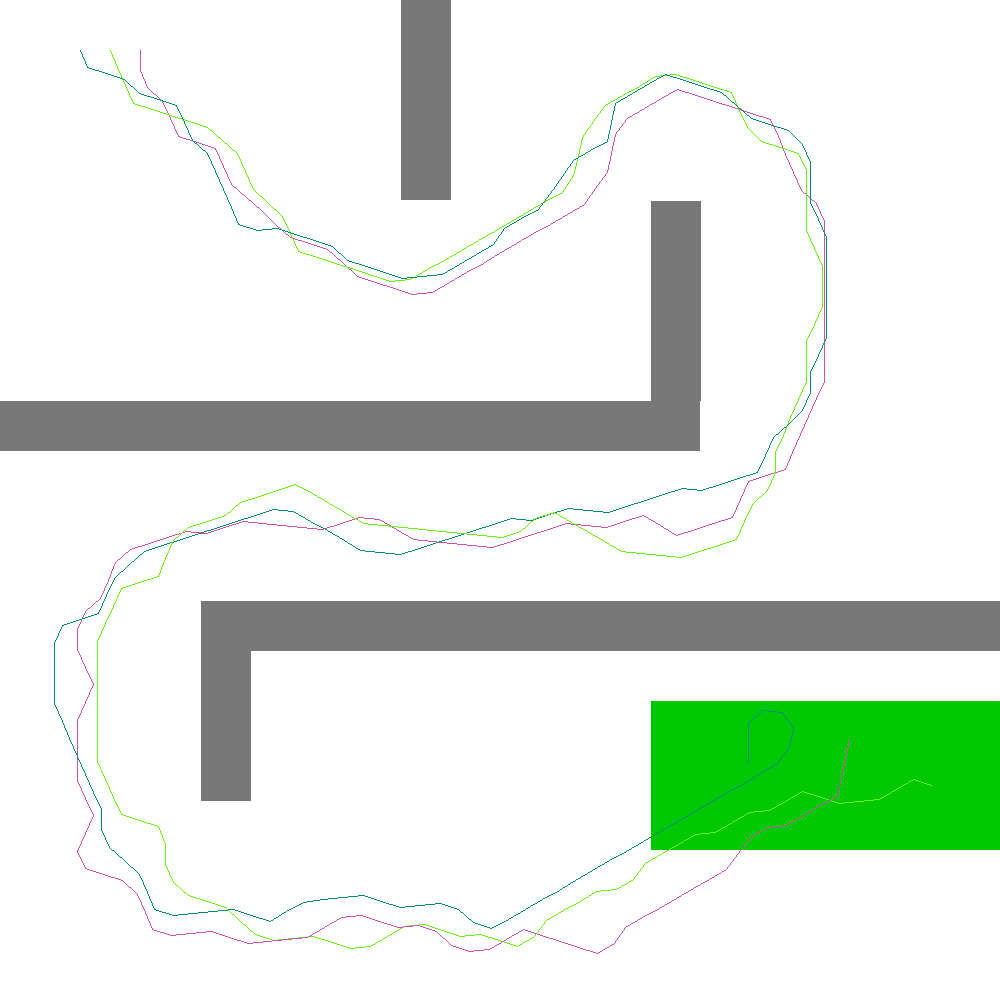
\includegraphics[scale=0.28]{obrazky/pathBeforeDubins}
\end{figure}


The best result of Dubins curves optimization (re-sampling of 20Hz)
is shown in \ref{fig:Path-after-Dubins}. As we can see, trajectories
are much shorter than trajectories before optimization in \ref{fig:Path-before-Dubins}.
On the beginning of trajectories, in the left upper corner of picture,
we can see much smoother curves than before optimization. This is
due to re-sampling to frequency 20Hz, which smooths trajectories. 

In real flight, it is undesirable to have trajectories tight to obstacles,
so obstacles are amplified before optimization. This can be seen in
\ref{fig:Path-after-Dubins} where UAVs keep certain distance from
the obstacles.

\begin{figure}


\caption{Path after Dubins curves optimization\label{fig:Path-after-Dubins}}


\centering{}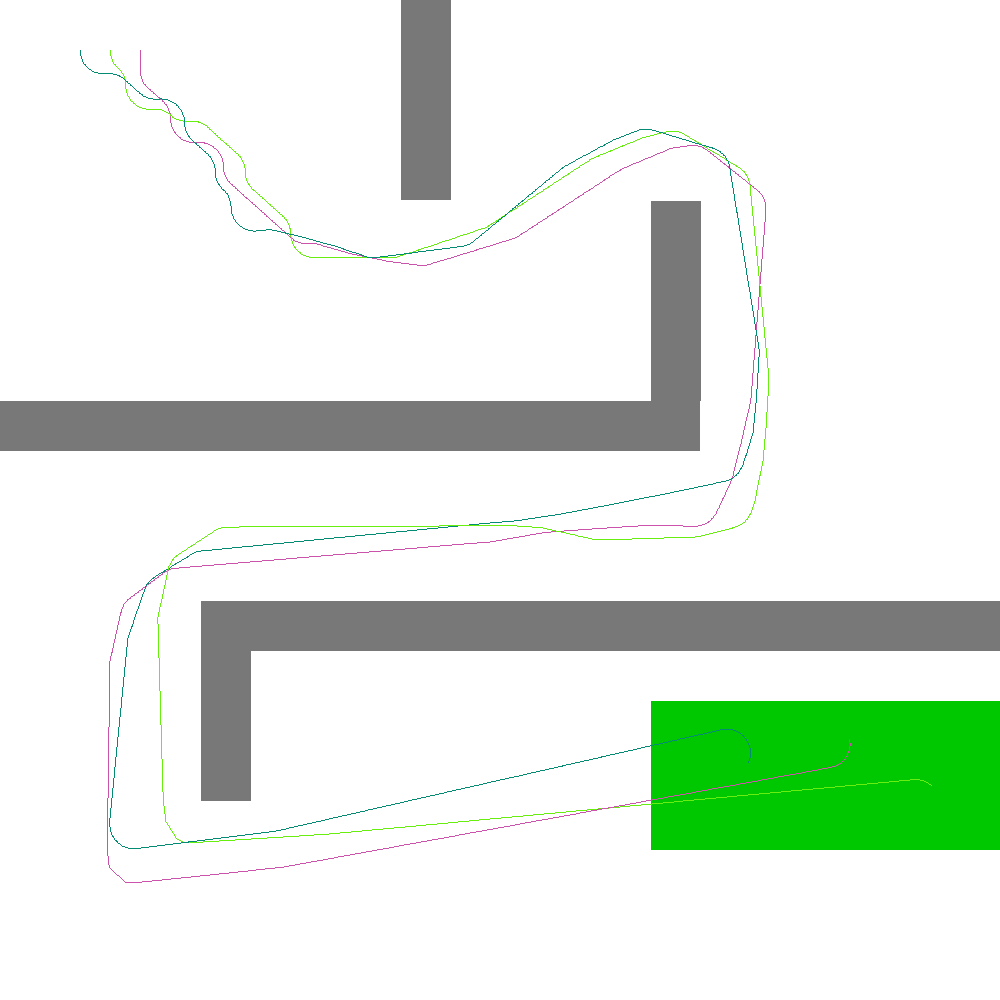
\includegraphics[scale=0.28]{obrazky/pathAfterDubins20Hz}
\end{figure}


As stated above, due to time and memory consumption, each optimization
is stopped after 150 iterations where optimization did not shorten
the path or when speed of path shortening was slower than 5\% of original
path length per 1000 iterations.

For each frequency, the optimization process was run 100 times to
obtain relevant results because of using random numbers during the
optimization.

Following table shows average total, minimal and maximal distance
of all trajectories from 100 optimizations after the re-sampling and
optimization.

\begin{table}
\caption{Re-sampling and optimization results\label{tab:Re-sampling-and-optimization}}


\begin{tabular}{|c|c|c|c|}
\hline 
Frequency {[}Hz{]} & Minimal distance {[}m{]} & Maximal distance {[}m{]} & Average distance {[}m{]}\tabularnewline
\hline 
\hline 
1 & 8582.18 & 8849.7 & 8721.2904\tabularnewline
\hline 
2 & 8311.65 & 8548.81 & 8430.23\tabularnewline
\hline 
4 & 8366.88 & 8393.09 & 8379.985\tabularnewline
\hline 
6 & 8248.9 & 8275.7 & 8262.3\tabularnewline
\hline 
8 & 8249.88 & 8378.51 & 8314.195\tabularnewline
\hline 
10 & 8286.22 & 8472.2 & 8379.21\tabularnewline
\hline 
12 & 8302.51 & 8309.2 & 8307.6613\tabularnewline
\hline 
14 & 8303.18 & 8303.18 & 8303.18\tabularnewline
\hline 
16 & 8363.92 & 8363.92 & 8363.92\tabularnewline
\hline 
18 & 8510.32 & 8510.32 & 8510.32\tabularnewline
\hline 
20 & 8194.22 & 8194.22 & 8194.22\tabularnewline
\hline 
\end{tabular}
\end{table}


The results are also shown in graph \ref{fig:Re-sampling-and-optimization}.
On the graph we can see that initial frequency 1 Hz has worst results
and the frequency 20 Hz has best results. We can also see that in
frequency 14 Hz and higher, all 100 iterations had same results, the
minimum, maximum and mean value are the same. But the second best
frequency in terms of minimal, maximal and mean value is 6 Hz and
even the worst optimization in 6 Hz has smaller total distance than
8 to 18 Hz. 

\begin{figure}


\caption{Re-sampling and optimization results graph \label{fig:Re-sampling-and-optimization}}


\centering{}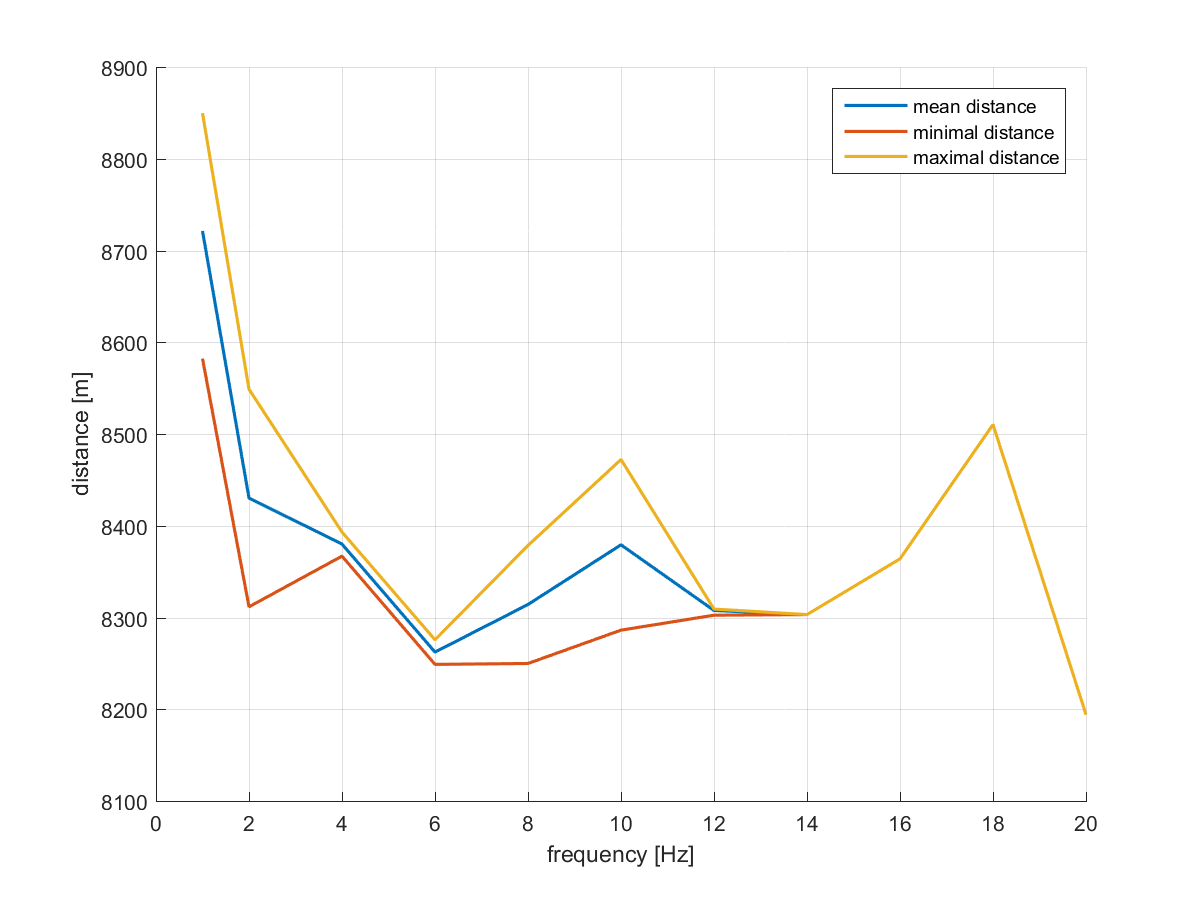
\includegraphics[scale=0.7]{obrazky/frequencyDependence}
\end{figure}


Depending on re-sampling frequency, the courses of optimization are
also different.

In \ref{fig:Time-course-of}, \ref{fig:Time-course-of-1} and \ref{fig:Time-course-of-2}
we can see mean values and standard deviations for different frequencies,
divided into three graphs for better readability. The vertical lines
are error bars, they show standard deviation during the optimization.
Because the error bars would be too dense if they were shown for each
iteration, only every 100th iteration is shown on graphs. For comparison,
on each graph is shown also frequency 1 Hz, the initial frequency
before re-sampling. As we can see, frequencies 14, 16, 18 and 20 Hz
have almost zero standard deviation and converge to lower value than
initial frequency. In frequency 10 Hz can be seen high standard deviation.
That means the optimization got stuck in local optimum and did was
not able to shorten any path for many iterations.

\begin{figure}


\centering{}\caption{Time course of optimization for 2 Hz, 4 Hz, 6 Hz\label{fig:Time-course-of} }
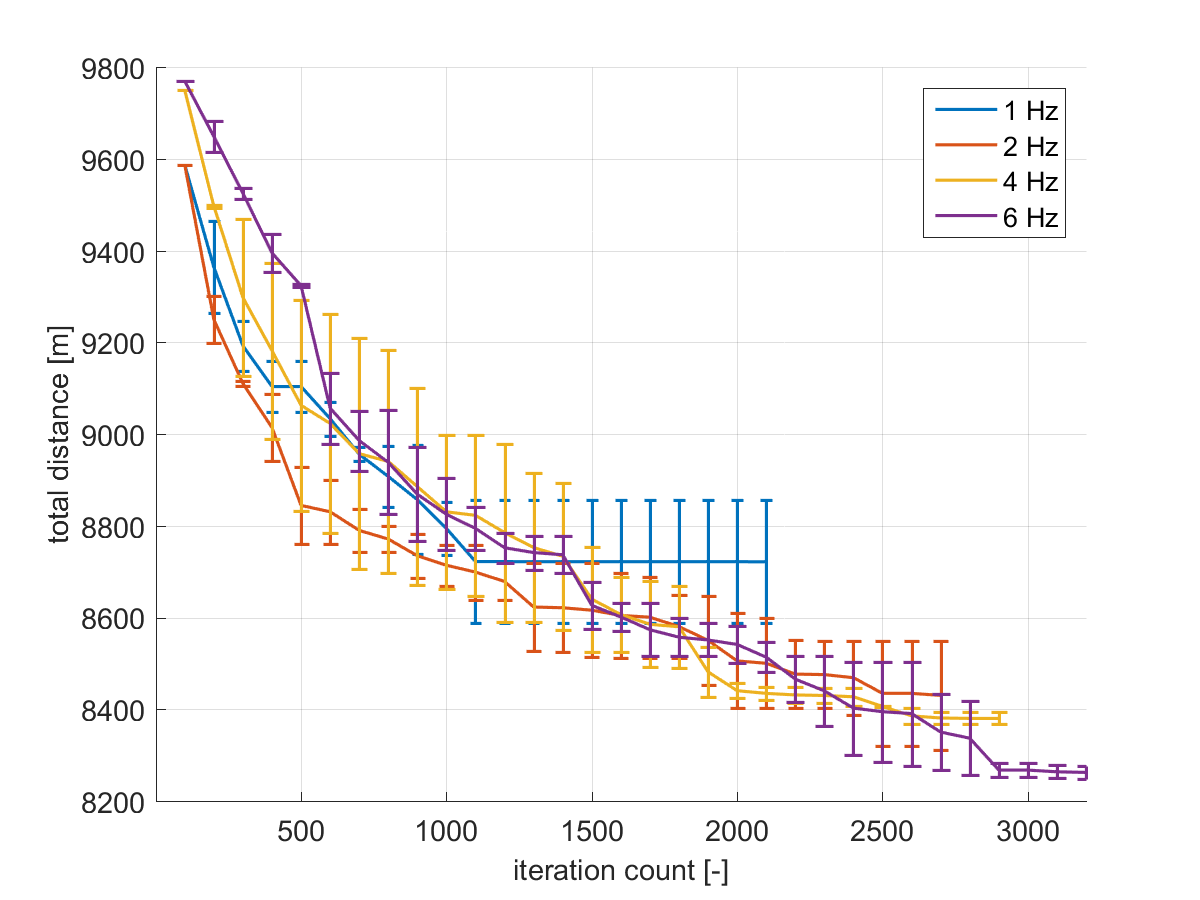
\includegraphics[scale=0.7]{obrazky/lowFrequenciesErrors}
\end{figure}


\begin{figure}


\caption{Time course of optimization for 8 Hz, 10 Hz, 12 Hz\label{fig:Time-course-of-1} }


\centering{}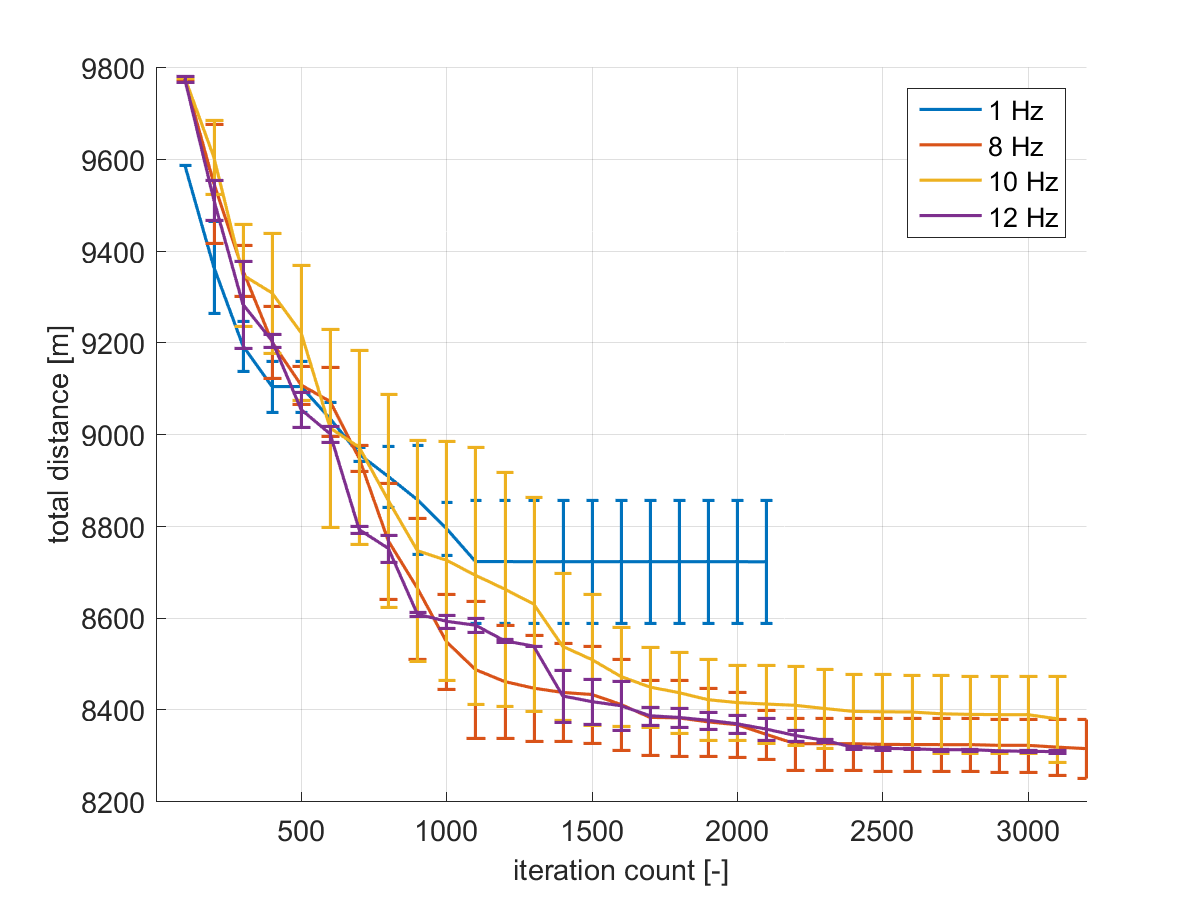
\includegraphics[scale=0.7]{obrazky/middleFrequenciesErrors}
\end{figure}


\begin{figure}


\caption{Time course of optimization for 14 Hz, 16 Hz, 18 Hz, 20 Hz\label{fig:Time-course-of-2} }


\centering{}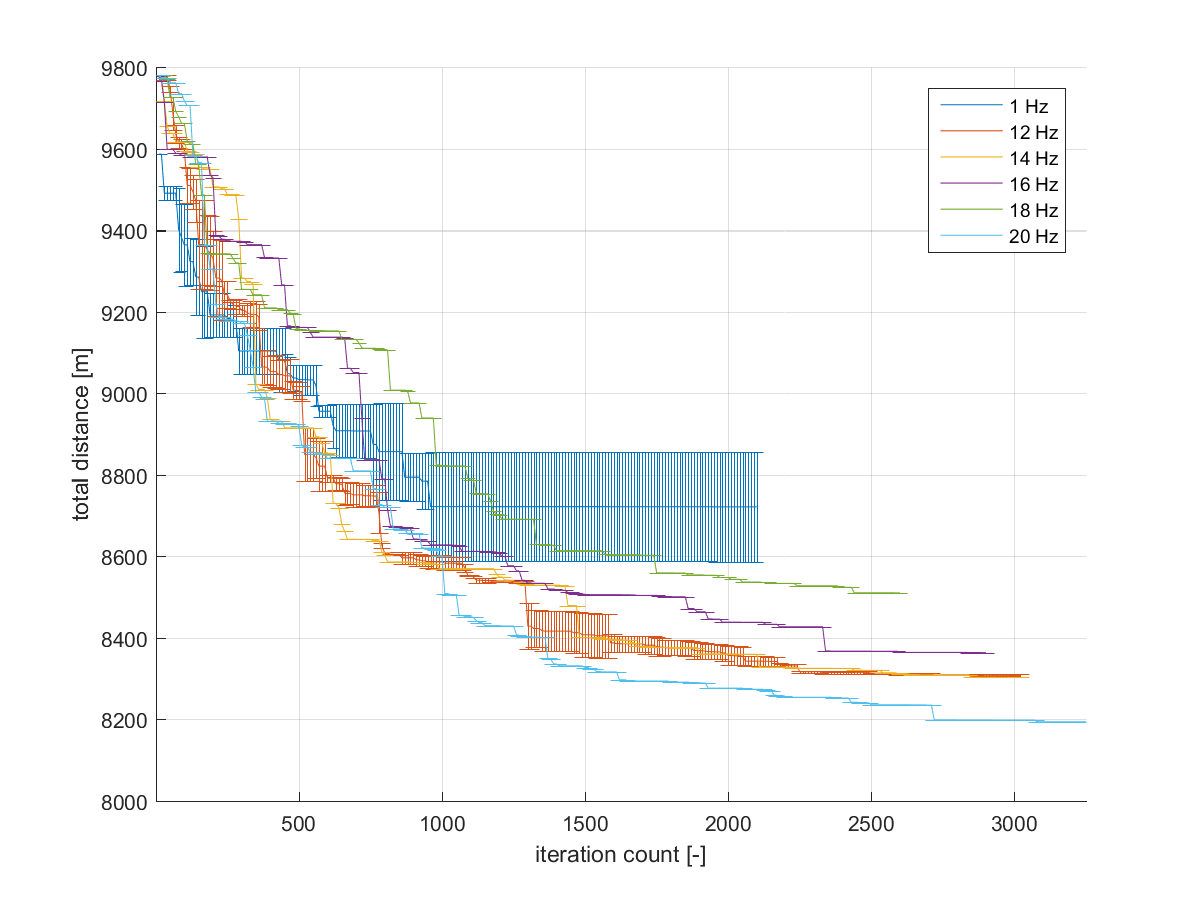
\includegraphics[scale=0.7]{obrazky/highFrequenciesErrors}
\end{figure}



\chapter[Covering more AoIs with one swarm]{Covering more AoIs with one swarm}


\chapter[V-REP simulations]{V-REP simulations}

V-REP is acronym for Virtual robot experimentation platform, a simulator
developed by Coppelia Robotics, providing an advanced environment
for testing and simulations of robots of all types. The V-REP environment
is free and open-souce for educational purposes and also has commercial
licence. The environment takes in account certain physical laws like
gravity, inertia or friction, which enables to truthfully verify applicability
for deployment of UAVs in the real world. V-REP has many build-in
models, but user can also create his own robot. V-REP enables to control
robots over API and has API clients for C, C++, Python, Java, Lua,
Matlab, Octave and Urbi. 


\section{UAV control and path simulation}

Python is convenient for fast prototyping and has native functions
for easy JSON parsing, which made it good choice for simulations of
generated trajectories in V-REP.

UAVs in V-REP can be controlled over remote API only by changing location
of their target. Then UAV tries to reach the location of its target.
Unfortunately, UAVs only follow location, with speed proportional
to distance. UAVs do not try to reach target and simultaneously to
have zero speed when reaching their target, which causes overshoot.
This fact leads to another disadvantage of UAV controller. When keeping
target in same distance and direction from UAV, the UAV increases
its speed, which causes overshoot when target changes its direction
to UAV. These overshoots were many times bigger than size of UAVs,
so they could not be ignored and had to be fixed.

During first, naive implementation, position of next state was set
as target position for UAV, but due to overshoot and large distances
between states UAVs failed to follow the trajectory. 

Another implementation linear interpolated trajectory between UAV
and its next state position and calculated target placed in line between
UAV and next state position, but in constant distance to UAV.

So the calculation was defined as follows
\[
\mathbf{X}\left(k+1\right)_{target}=\mathbf{X}\left(k\right)_{UAV}+\frac{\left(\mathbf{X}\left(k\right)_{ns}-\mathbf{X}\left(k\right)_{UAV}\right)}{\left\Vert \mathbf{X}\left(k\right)_{ns}-\mathbf{X}\left(k\right)_{UAV}\right\Vert }\cdot const
\]
where $\mathbf{X}\left(k\right)_{UAV}$ is UAV position in k-th iteration
of simulation, $\mathbf{X}\left(k\right)_{ns}$ is position of next
state in planned path in k-th iteration, $\mathbf{X}\left(k+1\right)_{target}$
is position of UAV target in (k+1)-th iteration and $const$ is constant
experimentally tuned, so the UAV does not move too fast nor too slow.
Too fast movements cause overshoot and too slow movements cause the
simulation to run for needlessly long time.

But a mentioned earlier, even this approach did not go well. In long
passages, where trajectory did not turn, UAVs increased their velocity
and inertia, which made them harder to turn. The problem of overshooting
is shown in figures \ref{fig:Map-with-UAV} and \ref{fig:UAV-overshoot}.
Overshoot is on the end of long passage in map \ref{fig:Map-with-UAV}.
Red and violet balls represent positions of next states and green
balls represent UAV targets. In the first image, we can see UAVs leaving
the narrow passage. As you can see in second and third image, positions
of next state are still, but because of constant distance of target
and UAV, the target is dragged by UAVs inertia.

This has been fixed by not updating the position of target when distance
between UAV and next state is bigger than in previous iteration and
the position of next state is still the same, so the equation describing
target position is
\[
\mathbf{X}\left(k+1\right)_{target}=\begin{cases}
if\left\Vert \mathbf{X}\left(k\right)_{ns}-\mathbf{X}\left(k\right)_{UAV}\right\Vert <\left\Vert \mathbf{X}\left(k-1\right)_{ns}-\mathbf{X}\left(k-1\right)_{UAV}\right\Vert \\
\land\mathbf{X}\left(k\right)_{ns}=\mathbf{X}\left(k-1\right)_{ns}\\
\mathbf{X}\left(k\right)_{UAV}+\frac{\left(\mathbf{X}\left(k\right)_{ns}-\mathbf{X}\left(k\right)_{UAV}\right)}{\left\Vert \mathbf{X}\left(k\right)_{ns}-\mathbf{X}\left(k\right)_{UAV}\right\Vert }\cdot const\\
else\\
\mathbf{X}\left(k\right)_{target}
\end{cases}
\]
. This prevents target from dragging by UAV with big inertia.

\begin{figure}
\begin{centering}
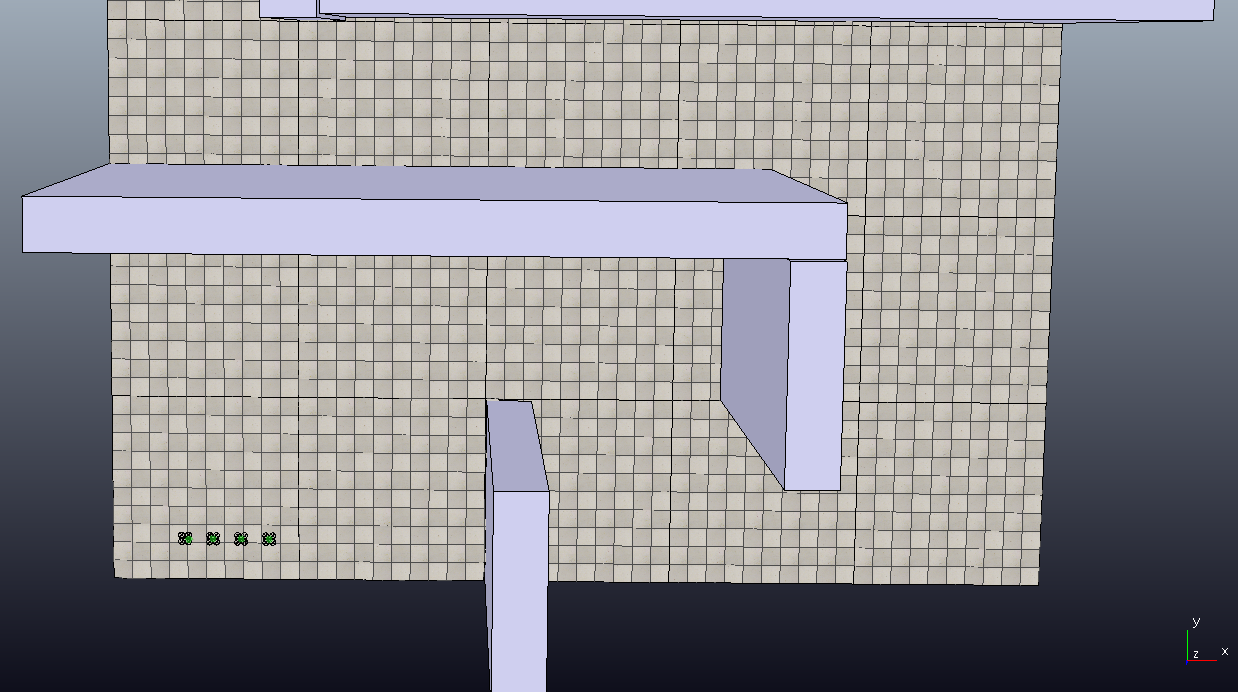
\includegraphics[scale=0.4]{obrazky/mapWithPassage}
\par\end{centering}

\caption{Map with UAV overshoot \label{fig:Map-with-UAV}}
\end{figure}


\begin{figure}
\begin{centering}
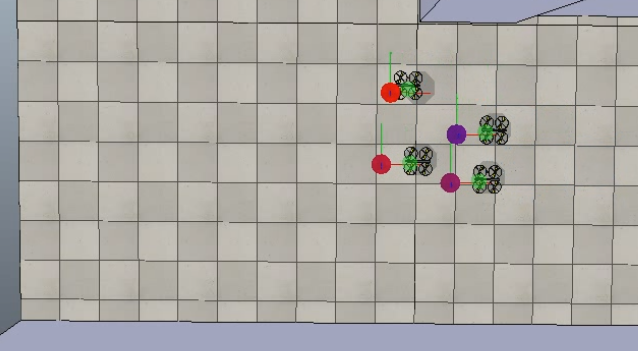
\includegraphics[scale=0.5]{obrazky/overshoot2}
\par\end{centering}

\begin{centering}
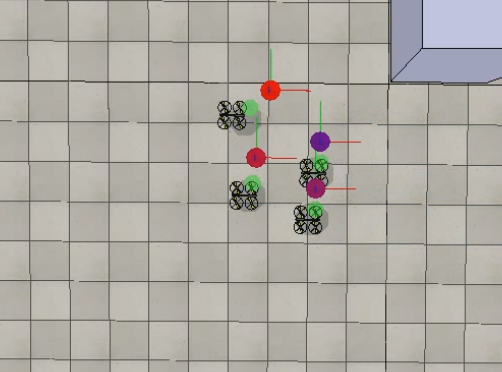
\includegraphics[scale=0.52]{obrazky/overshoot3_2}~~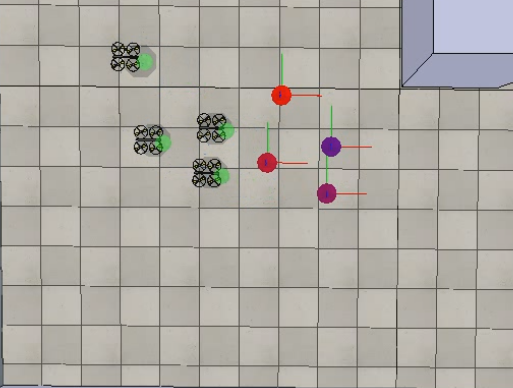
\includegraphics[scale=0.5]{obrazky/overshoot4}
\par\end{centering}

\caption{UAV overshoot\label{fig:UAV-overshoot}}


Here can be seen 3 iterations. Next state is changed during 
\end{figure}



\chapter[Implementation]{Implementation}

This part will cover implementation of algorithm, which was used for
simulations. Whole codebase in C++ can be found at \href{https://github.com/racinmat/AutonomousSurveillanceBachelorThesis}{this github repository}.
Next to the C++ program, I also created some CLI scripts in PHP, for
drawing map and paths from the JSON representation, batch running
of Dubins curves optimization and other useful stuff. These can be
seen at \href{https://github.com/racinmat/UAVUtils}{this github repository}.
V-REP simulations were made by communicating with V-REP through remote
API, the client is written in Python and can be seen \href{https://github.com/racinmat/VRepPathBuilder}{here}.


\section{External libraries}

In implementation are used some external libraries. Every used library
is mentioned here.\href{http://www.boost.org/}{Boost libraries} is
used for smart pointers, libraries for Dubins curves are from Master
Thesis by Petr Váňa\cite{Vana2015}. Generating of JSON from C++ object
is done via \href{http://www.codeproject.com/Articles/20027/JSON-Spirit-A-C-JSON-Parser-Generator-Implemented}{Json Spirit}
library. Another external library is \href{http://gamma.cs.unc.edu/V-COLLIDE/}{V-Collide}
from The University of North Carolina at Chapel Hill. 

Because V-Collide sources were written in 1997 and because I used
C++11 compiler to compile my source codes, I had to rewrite part of
this library for compatibility and to make public API easier to use.
Modifications can be seen in \href{https://github.com/racinmat/VCollide2}{this github repository}. 

Last used external library is QT, which was used to create platform
independent GUI.


\section{Code structure and services}

Here is shown brief UML scheme demonstrating dependency diagram of
codebase. To keep diagram simple, only services are displayed, other
classes, which are not services, were left out for lucidity. Diagram
was generated using software \href{http://staruml.io/}{StarUML}

\begin{figure}
\caption{Dependency diagram \label{fig:Dependency-diagram}}


\centering{}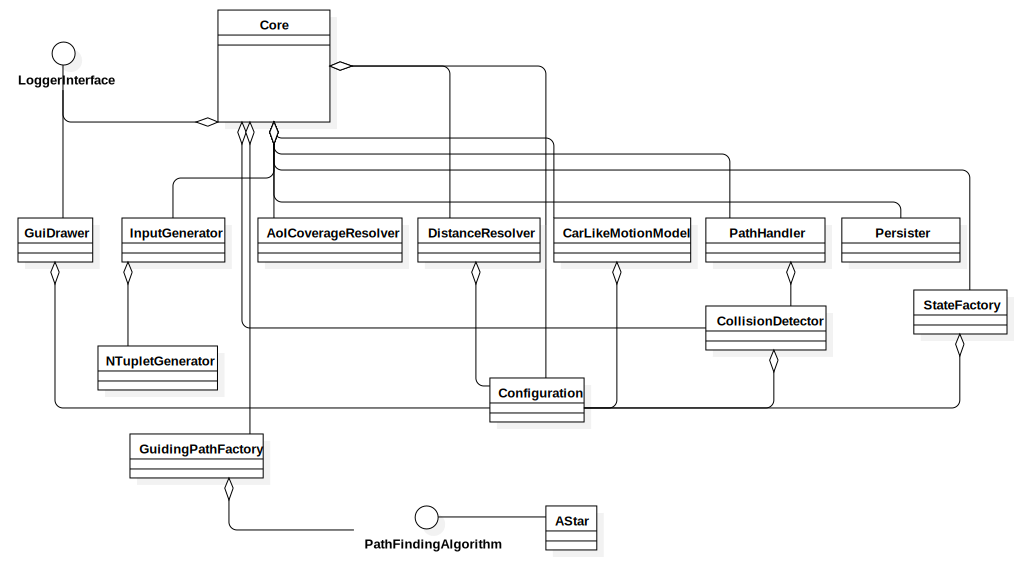
\includegraphics[scale=0.4]{obrazky/umlSchema}
\end{figure}


Core class holds core of whole Application and has all other classes
as dependencies, as is shown in image \ref{fig:Dependency-diagram}. 

As mentioned in \ref{chap:Algorithm} chapter Configuration is DTO
for all configuration variables, but to keep reasonable amount of
classes, Configuration is also service, which delegates all configuration
changes from GUI to Core class. Configuration and GuiDrawer implementation
LoggerInterface are the only connections between Core and GUI.

State factory creates State classes according to Factory pattern.
State class represents state in RRT-Path algorithm. State has coordinates
and rotations for all UAVs.

Persister persists found path to JSON using Json Spirit library.

PathHandler serves as utils class for manipulations with path (vector
of State classes).

CarLikeMotionModel holds motion model algorithm.

InputGenerator is used to generate inputs to motion model.

NTupletGenerator only generates variation with repeating for given
input.

DistanceResolver counts distances between two states and distance
of path.

AoICoverageResolver determines cost function for states,where all
UAVs are in AoIs.

GuidingPathFactory is wrapper for PathFindingAlgorithm interface and
is used by Core to find guiding path. 

Implementation of PathFindingAlgorithm is AStart class.

\bibliographystyle{plainnat}
\phantomsection\addcontentsline{toc}{chapter}{\bibname}\bibliography{bibliography}


\cleardoublepage{}
\end{document}
